% Radio Science (AGU) manuscript draft — Paper 2
% Prefer agujournal2025.cls (copied from Paper 1 draft) or agujournal2019.cls from AGU.
%
\documentclass[draft]{agujournal2019}
\usepackage{amsmath}
\usepackage{graphicx}
\usepackage{url}
\usepackage{lineno}
\linenumbers

\graphicspath{{../analysis/figures/}}

\journalname{Radio Science}

\begin{document}

\title{Kinematic Oscillating Sheath Boundary in Three-Dimensional Plasma Fluid FDTD: Isolating Song's Moving-Boundary Coupling Without Particle-in-Cell}

\authors{A. Author\affil{1}, B. Author\affil{1}}

\affiliation{1}{Institution, City, Country}

\correspondingauthor{A. Author}{author@example.edu}

\begin{keypoints}
\item A prescribed oscillating sheath radius is implemented in three-dimensional plasma fluid FDTD.
\item At 700 kHz the oscillating feed impedance lies far outside the static radius brackets.
\item Staircased kinematic motion can change feed loading beyond quasi-static sheath thickness.
\end{keypoints}

\begin{abstract}
High-voltage antennas in plasma develop electron-depleted sheaths whose radius can oscillate at the drive frequency.
Song's analytic treatment links radiation and feed loading to the moving sheath boundary through a current proportional to the boundary velocity.
Particle-in-cell (PIC) models recover related self-consistent sheath dynamics but are costly in three dimensions.
Here we introduce a kinematic sheath in a plasma fluid finite-difference time-domain (PF-FDTD) solver: the depleted-radius history \(r_s(t)\) is prescribed, while Maxwell and fluid equations remain unchanged.
A single-tone pilot at \(700\,\mathrm{kHz}\) (\(f_p=2\,\mathrm{MHz}\)) compares oscillating \(r_s(t)=4+\sin(\omega t)\) cells against static jackets of width 4 and 5 cells.
Phasor feed impedance for the oscillating case is strongly offset from the static bracket segment in the complex plane (\(|\Delta Z|\) to the segment \(\sim 9\times\) the bracket span), with \(\mathrm{Re}\{Z\}\) rising from \(\sim 1.4\text{--}1.8\times 10^{4}\,\Omega\) (static) to \(\sim 7.3\times 10^{4}\,\Omega\) (oscillating).
Time-domain current shows staircasing-related high-frequency structure absent in the static controls.
The result indicates that prescribed boundary motion can change feed loading beyond quasi-static thickness sampling in this engine, motivating \(\Delta r\) scans and caution about staircased updates before self-consistent charging work.
\end{abstract}

\section*{Plain Language Summary}
Radio antennas in space plasmas are surrounded by a low-density sheath.
When the antenna voltage is large, that sheath can breathe in and out each radio cycle, and the motion itself can help launch waves or change how the antenna loads.
Fully kinetic particle simulations can capture this breathing but are expensive in three dimensions.
We prescribe the sheath size as a known oscillating function of time inside an existing fluid electromagnetic code, then compare the antenna voltage and current to cases where the sheath thickness is fixed.
In a first controlled test, the oscillating case produced a feed impedance clearly different from either fixed thickness, showing that boundary motion can matter even without self-consistent charging.

\section{Introduction}
\label{sec:intro}

A depleted sheath between a metallic antenna and the ambient plasma inserts a largely reactive series impedance and can dominate feed behavior at ionospheric and magnetospheric radio frequencies
\cite{balmain1964,liu_sheath,song2007,tu2008}.
For high-voltage whistlers and related transmitters, Song~\cite{song2007} argued that the sheath is nearly electron-free and that the oscillating outer radius \(r_s(t)\) supplies a radiation current tied to \(\dot{r}_s\).
Tu et al.~\cite{tu2008} later examined the same problem with one-dimensional PIC, improving reactance agreement relative to Song's analytics.

Three-dimensional plasma fluid FDTD (PF-FDTD) can already impose a \emph{static} volumetric density hole of width \(S_d\) around a thin-wire dipole and measure feed impedance
\cite{ward2006}.
Campaign work with that prescribed jacket showed strong series-capacitance loading once the hole was seeded from the conductor surface rather than from a plasma-on mask
(companion campaign chronicle; static capacitance study in preparation).
Varying static \(S_d\) samples different quasi-steady thicknesses but does not represent Song's moving-boundary current.

This paper asks a narrower question: if \(r_s(t)\) is \emph{prescribed} to oscillate at the drive frequency inside the same Maxwell--fluid core, do feed diagnostics show \(\omega\)-locked differences attributable to \(\dot{r}_s\) beyond static jackets of thickness \(r_{s0}\) and \(r_{s0}+\Delta r\)?
A positive signature would support investing in self-consistent charging; a controlled null result would still clarify the limits of kinematic sheath models in fluid FDTD.

\section{Model and Methods}
\label{sec:methods}

\subsection{Plasma fluid FDTD}
\label{sec:pffdtd}

We advance Maxwell's equations on a staggered Yee grid coupled to multi-species cold/warm fluid continuity and momentum equations following the PF-FDTD formulation of Ward~\cite{ward2006}.
Plasma--Maxwell coupling is masked by a conductivity field \(\mathrm{SIG}\) on free-space cells; conductors are encoded by permittivity flags \(\mathrm{ER}_*=0\).
Feed voltage and current are recorded at the dipole gap for impedance diagnostics.
Unless noted, the plasma frequency, collision ratio, and grid match the companion static-sheath campaign (\(f_p=2\,\mathrm{MHz}\), \(\Delta x=0.04\,\mathrm{m}\)).

\subsection{Kinematic sheath radius}
\label{sec:rst}

The ambient density \(N_0(\mathbf{r})\) is depleted to a floor fraction inside a staircased neighborhood of the PEC antenna.
For the oscillating case we adopt
\begin{equation}
r_s(t)=r_{s0}+\Delta r\sin(2\pi f_{\mathrm{osc}}t+\phi),
\label{eq:rst}
\end{equation}
with \(r_{s0}\) and \(\Delta r\) expressed in grid cells.
A PEC-seeded integer distance field is computed once out to \(S_{\max}=\lceil r_{s0}+|\Delta r|\rceil\).
At each time step the integer threshold \(S_d(t)=\mathrm{round}[r_s(t)]\) is applied only when it changes, restoring bulk \(N_0\) outside the instantaneous hole and flooring fluid density inside newly covered cells.
When \(\Delta r=0\), the static sheath path is unchanged, preserving continuity with prior static-\(S_d\) runs.

Oscillation frequency defaults to the RF drive; phase \(\phi\) is a free control.
Song's \(r_s^2(t)\) law is deferred; the sinusoid is the minimal mechanism probe.

\subsection{Experimental design}
\label{sec:design}

For a single CW tone below \(f_p\) we compare three runs: static \(r_{s0}\), static \(r_{s0}+\lceil\Delta r\rceil\), and oscillating equation~\eqref{eq:rst}.
Success metrics are (i)~an \(\omega\)-locked difference in feed \(Z\) for the oscillating case relative to both static brackets, (ii)~sensible scaling with \(\Delta r\), and (iii)~phase relations between boundary motion and feed \(V\)/\(I\) where interpretable.
Matching Tu PIC reactance is \emph{not} required.

The pilot reported here uses \(f=700\,\mathrm{kHz}\), \(r_{s0}=4\), \(\Delta r=1\), \(\phi=0\), \(4.3\times 10^{5}\) time steps, and phasor \(Z=V/I\) estimated from the last half of each voltage/current record.

\section{Results}
\label{sec:results}

Table~\ref{tab:pilotZ} lists fundamental-frequency phasors.
The two static jackets differ modestly (\(|Z_5-Z_4|\approx 6.0\times 10^{3}\,\Omega\)), as expected for a one-cell thickness change.
The oscillating case does \emph{not} fall between them: \(\mathrm{Re}\{Z\}\) increases by a factor of about four relative to the static mean radius, while \(\arg(Z)\) moves from \(\approx -70^\circ\) to \(\approx -31^\circ\).
In the complex plane (Figure~\ref{fig:Zcomplex}), the distance from the oscillating phasor to the static bracket segment is \(\approx 5.6\times 10^{4}\,\Omega\), about nine times the bracket span.

\begin{table}
\caption{Pilot phasor feed impedance at \(700\,\mathrm{kHz}\) (last 50\% of each trace).}
\label{tab:pilotZ}
\centering
\begin{tabular}{lcccc}
\hline
Case & \(\mathrm{Re}\{Z\}\) ($\Omega$) & \(\mathrm{Im}\{Z\}\) ($\Omega$) & $|Z|$ ($\Omega$) & $\arg Z$ (deg) \\
\hline
Static $r_{s0}=4$ & $1.76\times 10^{4}$ & $-4.75\times 10^{4}$ & $5.06\times 10^{4}$ & $-69.7$ \\
Static $r_{s0}+1=5$ & $1.42\times 10^{4}$ & $-4.26\times 10^{4}$ & $4.49\times 10^{4}$ & $-71.6$ \\
Oscillating $\Delta r=1$ & $7.31\times 10^{4}$ & $-4.32\times 10^{4}$ & $8.49\times 10^{4}$ & $-30.6$ \\
\hline
\end{tabular}
\end{table}

\begin{figure}
\noindent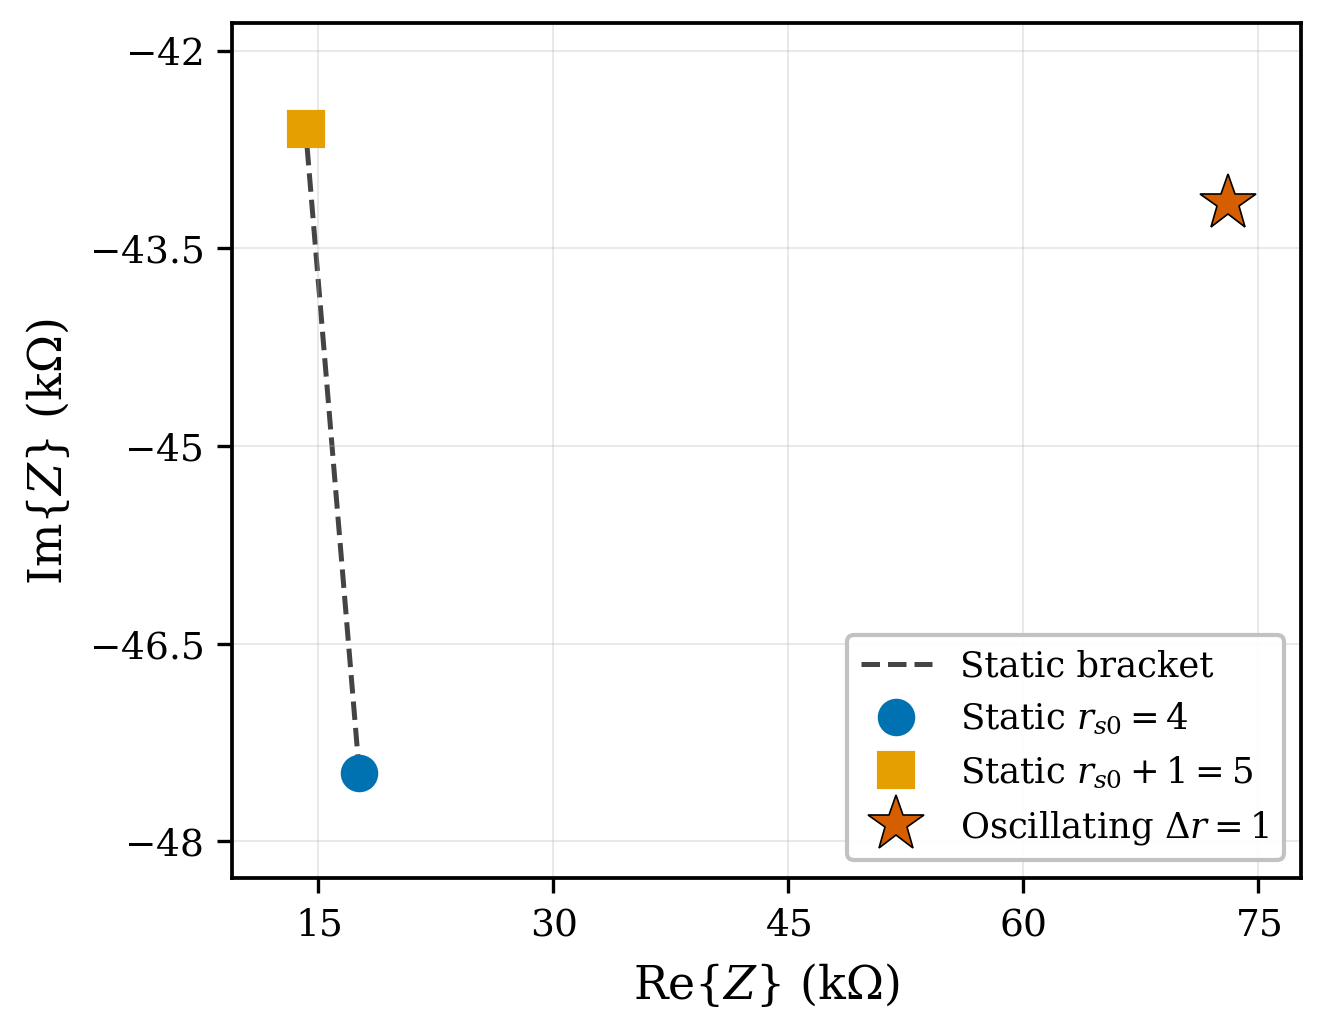
\includegraphics[width=\textwidth]{pilot_Z_complex.png}
\caption{Complex-plane phasor \(Z\) at \(700\,\mathrm{kHz}\). The dashed line is the static bracket between \(r_{s0}=4\) and \(r_{s0}+1=5\). The oscillating point lies far off that segment.}
\label{fig:Zcomplex}
\end{figure}

Figure~\ref{fig:VI} shows the last few drive cycles.
Voltage waveforms overlay (voltage drive).
Static currents remain nearly sinusoidal; the oscillating-sheath current develops large high-frequency spikes coincident with integer radius updates.
Component bars (Figure~\ref{fig:Zbars}) emphasize that the primary excursion is in \(\mathrm{Re}\{Z\}\) and \(|Z|\), not a small interpolation of the static reactances.

\begin{figure}
\noindent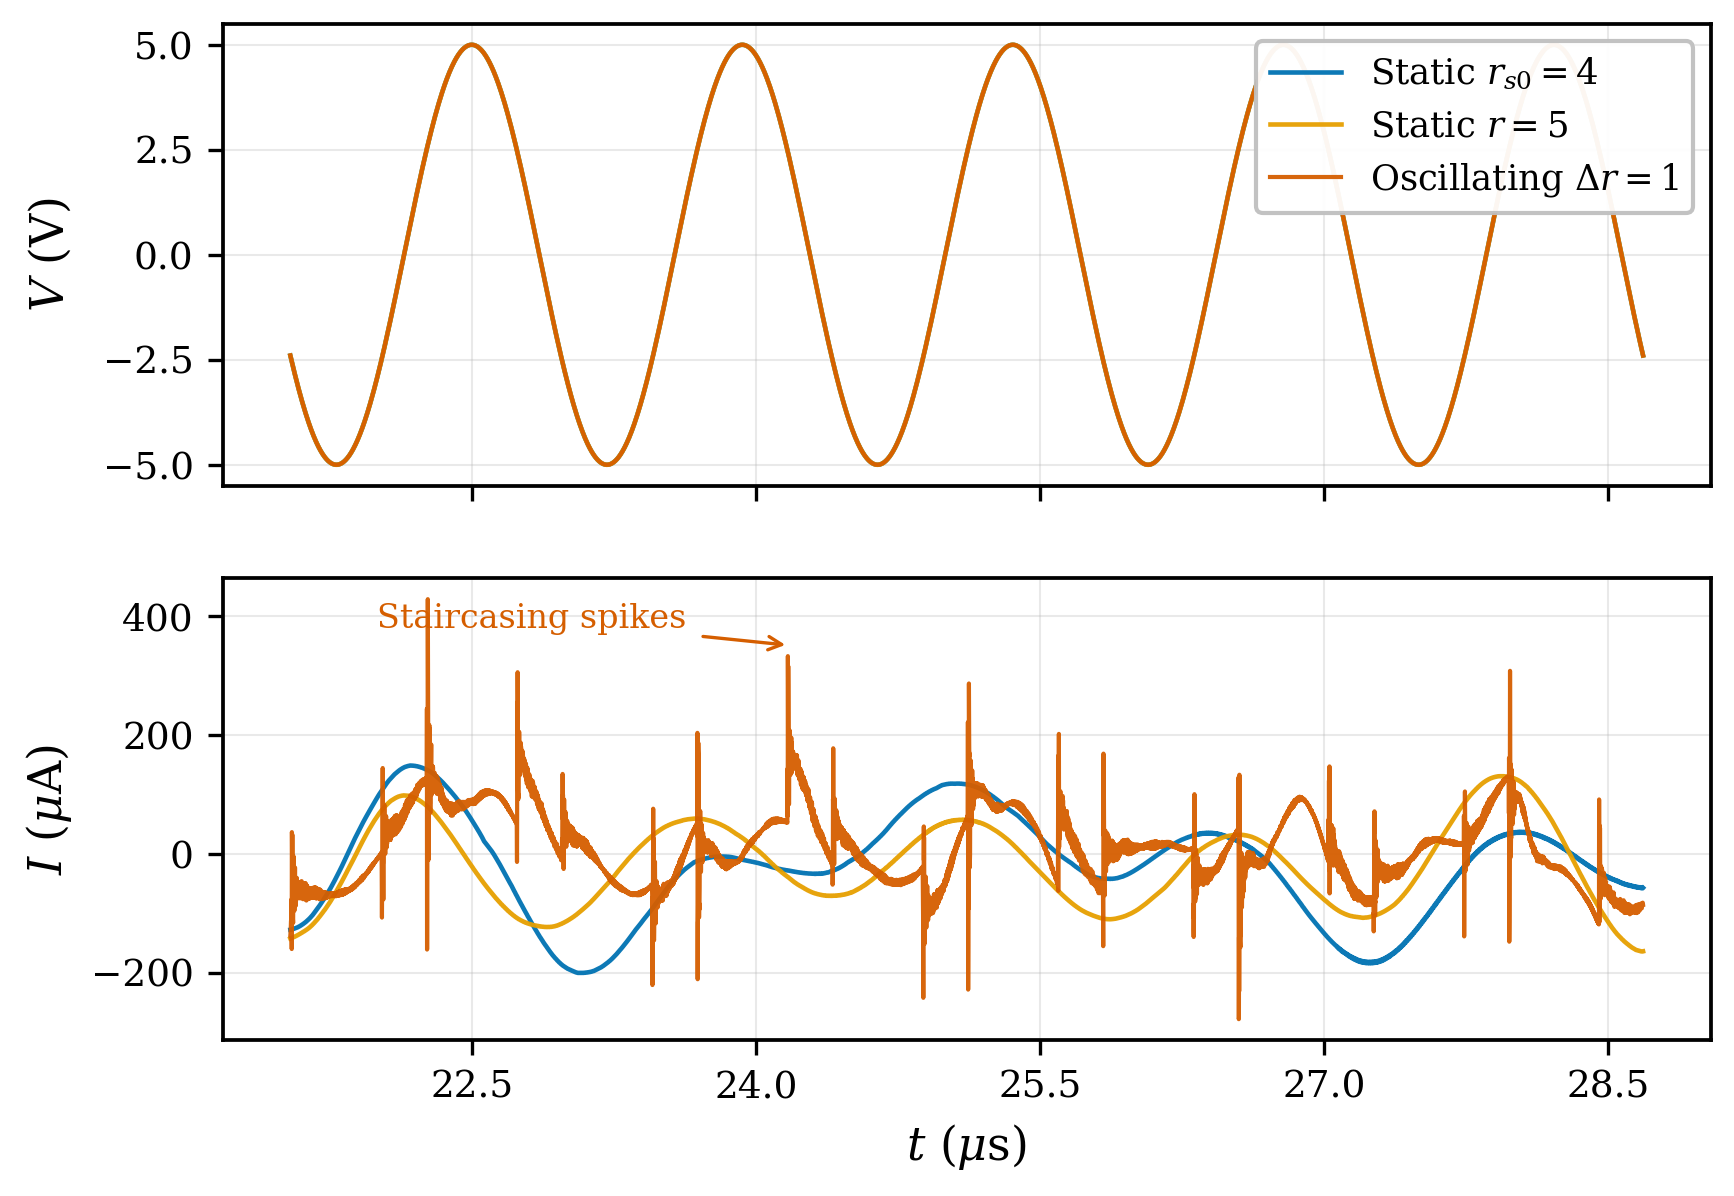
\includegraphics[width=\textwidth]{pilot_VI_last_cycles.png}
\caption{Late-time feed voltage and current. Oscillating-sheath current shows staircasing-related spikes absent in the static controls.}
\label{fig:VI}
\end{figure}

\begin{figure}
\noindent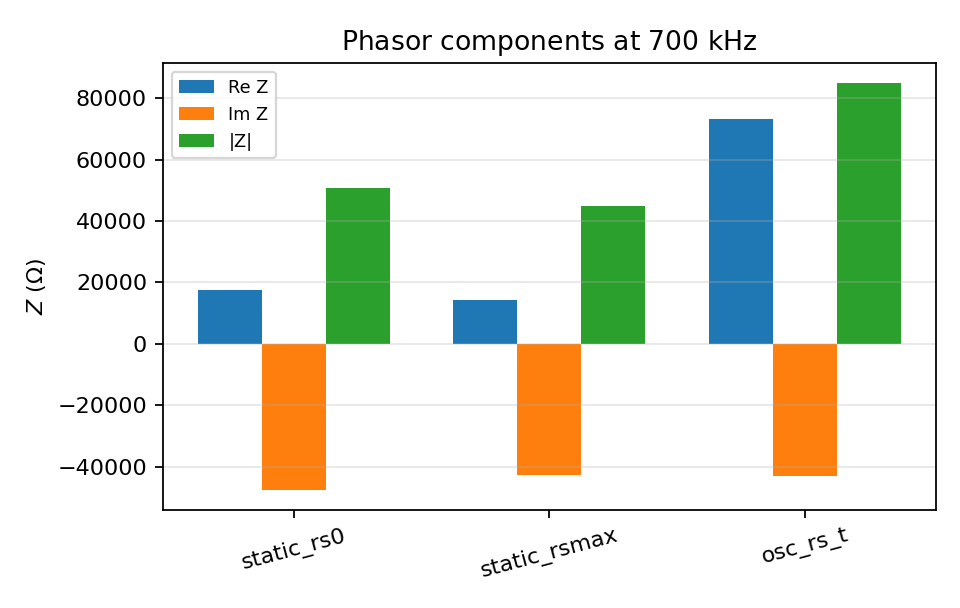
\includegraphics[width=0.85\textwidth]{pilot_Z_bars.png}
\caption{Phasor \(\mathrm{Re}\{Z\}\), \(\mathrm{Im}\{Z\}\), and \(|Z|\) for the three pilot cases.}
\label{fig:Zbars}
\end{figure}

\section{Discussion}
\label{sec:discussion}

The pilot rejects the null hypothesis that kinematic \(r_s(t)\) is indistinguishable from quasi-static sampling of \(r_{s0}\) and \(r_{s0}+\Delta r\) at this tone and amplitude.
That is the central Paper~2 question in miniature: prescribed boundary motion changes the feed diagnostic beyond thickness brackets.

Two caveats are essential.
First, the staircased integer mask injects impulsive current structure (Figure~\ref{fig:VI}); part of the fundamental phasor shift may be numerical rather than a clean Song \(\dot{r}_s\) continuum current.
Second, the fluid density floor is not a strictly electron-free sheath, and no self-consistent bias is solved.
Therefore we interpret the result as \emph{evidence that kinematics matter in this engine}, not as quantitative validation of Song~\cite{song2007} or Tu et al.~\cite{tu2008}.

Next steps are a \(\Delta r\) amplitude scan, phase sweeps, optional sub-cell or filtered radius updates to reduce staircasing noise, and only then a go/no-go decision on self-consistent charging (Paper~3).

\section{Conclusions}
\label{sec:conclusions}

We implemented a prescribed oscillating sheath boundary in three-dimensional PF-FDTD and compared it to static radius brackets at \(700\,\mathrm{kHz}\).
The oscillating feed impedance lies well outside the static bracket segment, with a large increase in \(\mathrm{Re}\{Z\}\) and reduced phase lag, while time-domain current shows staircased update spikes.
Kinematic sheath motion is therefore detectable in this solver; quantitative Song/Tu fidelity and the role of staircasing remain open and motivate controlled parameter scans before self-consistent extensions.

%%

\acknowledgments
The authors thank collaborators on the PF-FDTD sheath campaign.
Funding statement to be added.

\section*{Open Research}
Pilot inputs and analysis scripts are in the project repository under \texttt{projects/tu2008-sheath/} (solver binary \texttt{pffdtd\_parallel\_rs\_t}, script \texttt{run\_paper2\_rs\_t\_pilot.ps1}, analyzer \texttt{analyze\_paper2\_pilot.py}).
Derived tables and figures are under \texttt{paper2\_oscillating\_sheath\_boundary/analysis/}.
Public archival deposit will accompany journal submission.

\bibliography{references}

\end{document}
